\documentclass[tikz,border=4pt]{standalone}
\usetikzlibrary{petri,positioning,arrows.meta}
\begin{document}
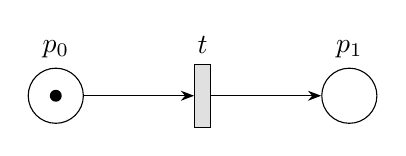
\begin{tikzpicture}[
  >=Stealth,
  every place/.style={draw,minimum size=7mm},
  every transition/.style={draw,fill=black!12,minimum width=2mm,minimum height=8mm},
  node distance=14mm
]
  \node[place,tokens=1,label=above:{$p_0$}] (input) {};
  \node[transition,right=of input,label=above:{$t$}] (step) {};
  \node[place,right=of step,label=above:{$p_1$}] (output) {};
  \draw[->] (input) -- (step);
  \draw[->] (step) -- (output);
\end{tikzpicture}
\end{document}
